%%%%%%%%%%%%%%%%%%%%%%% file template.tex %%%%%%%%%%%%%%%%%%%%%%%%%
%
% This is a general template file for the LaTeX package SVJour3
% for Springer journals.          Springer Heidelberg 2010/09/16
%
% Copy it to a new file with a new name and use it as the basis
% for your article. Delete % signs as needed.
%
% This template includes a few options for different layouts and
% content for various journals. Please consult a previous issue of
% your journal as needed.
%
%%%%%%%%%%%%%%%%%%%%%%%%%%%%%%%%%%%%%%%%%%%%%%%%%%%%%%%%%%%%%%%%%%%

\RequirePackage{fix-cm}
%\documentclass[twocolumn]{svjour3}          % twocolumn
\documentclass[smallextended]{svjour3}          % twocolumn

\smartqed  % flush right qed marks, e.g. at end of proof

\usepackage{graphicx} % adjustbox loads it
\usepackage{epstopdf} % loads eps
\usepackage[normalem]{ulem}

% insert here the call for the packages your document requires
\usepackage{geometry}
\usepackage[export]{adjustbox}
\usepackage[labelfont=bf, labelsep=space]{caption}
%\usepackage{subcaption}
\usepackage{subfig}
\usepackage[utf8]{inputenc}
\usepackage{amssymb}
\usepackage{amsmath} 

\usepackage{natbib} % enables author year and other citation styles
\usepackage[bookmarks,bookmarksopen,bookmarksdepth=2]{hyperref} % active links
\hypersetup{backref,
	colorlinks=true,
	citecolor=blue,
	linkcolor=blue}

\usepackage{tikz} % graphics,
\usetikzlibrary{fit,positioning} % tikz elements positioning
\usepackage{soul} % annotations


\DeclareMathOperator*{\argmin}{arg\,min}

\newcommand\alberto[1]{\textcolor{red}{#1}}

%\DeclareGraphicsRule{.tif}{png}{.png}{`convert #1 `dirname #1`/`basename #1 .tif`.png}

\graphicspath{ {./img/} }
\DeclareMathOperator*{\argmax}{arg\,max}
\journalname{}

\begin{document}
\title{You are the way you structurally talk: Structural-temporal neighborhoods of posts to characterize users in online forums}

\author{Alberto Lumbreras \and
        Julien Velcin  \and\\
        Marie Guégan \and
        Bertrand Jouve
}

\institute{Alberto Lumbreras \and Marie Guégan \at
		   Technicolor\\
           975 Avenue des Champs Blancs, \\35576 Cesson-Sévigné,\\ France\\
           \email{alberto.lumbreras@technicolor.com}\\
           \email{marie.guegan@technicolor.com}
           \and
           Julien Velcin \at
           Laboratoire ERIC, Université de Lyon,\\
           5, avenue Pierre Mendès France, 69676 Bron,\\ France\\
           \email{julien.velcin@univ-lyon2.fr}
		  \and
           Bertrand Jouve \at
           Université de Toulouse; UT2; FRAMESPA/IMT; 5 allée Antonio Machado, 31058 Toulouse, cedex 9\\
           CNRS; FRAMESPA; F-31000 Toulouse\\
           CNRS; IMT; F-31000 Toulouse\\ France\\     
           \email{jouve@univ-tlse2.fr}
}

\date{Draft date: \today}
% The correct dates will be entered by the editor

\maketitle

%%%%%%%%%%%%%%%%%%%%%%%%%%%%%%%%%%%%%%%%%%%%%%%%%%%%%%
%%%%%%%%%%%%%%%%%%%%%%%%%%%%%%%%%%%%%%%%%%%%%%%%%%%%%%
\section{Introduction}\label{sec:introduction}

The popularization of online forums has brought a growing interest on their underlying dynamics. As any other complex system, an the dynamic of online forums can be studied at different levels, from the more macro to the most micro. Macro dynamics are, for instance, the evolution of some global properties such as its diameter, or its distribution degree. Micro dynamics are, for instance, the triadic motifs that represent local phenomena such as transitivity (friends of my friends are also my friends).

An interesting question in online communities is that concerning roles. In sociology, roles are generally seen as the set of expected behaviours that are attached  to a position in the community. Extrapoliting the notion of role, some researchers have looked for roles in online forums. Some others have tried to detect the roles and the users who hold that roles.

Roles can also be studied from the macro or the micro perspective. If studied from the macro, we can analyse the number of users, the percentage of replied post, its centrality in the network, and  so forth.

In this paper, we focus on the analyse of roles at a micro level, and more specifically at the discussion level. We would like to answer the following question: are there different types of users in terms of the kind of conversation they participate in?


Our intuition is that some users like participating in some kind of discussion rather than other. Certainly, an analysis of the textual content will tell us much about a discussion. However, due to the huge diversity of topics, vocabulary, and the difficulty of current algorithms to capture the language subtleties such as humor, irony, or changing contexts, we turn our attention towards the structure of the discussions. More precisely, we analyze the local graph structure in which a user post in embedded, in the hope that this structure will be meaningful since it also reflects the kind of conversation in that part of the thread.

Formally, these local graphs are known as neighborhoods.


The remaining of the paper is as follows. First we will introduce our representation of online discussions. Then we will explain our concept of structural neighbourhood. Then we will apply this to the clustering of users and we will analyze the clusters. Finally, we will attemp to study whether these roles have predictive power.


\section{Discussion trees}
A natural way to represent a conversation thread is a tree graph where vertex represent posts and edges represent replies from some post to another. The tree is rooted at the post who started the thread. This representation allows to apply the mathematical toolbox of graph theory. Figure~\ref{fig:trees} shows some real examples of trees in a Reddit\footnote{www.reddit.com} forum.

\begin{figure}
	\centering
	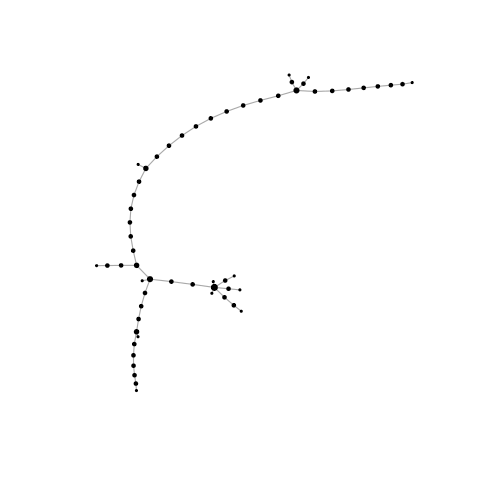
\includegraphics[width=0.32\textwidth]{tree1}
	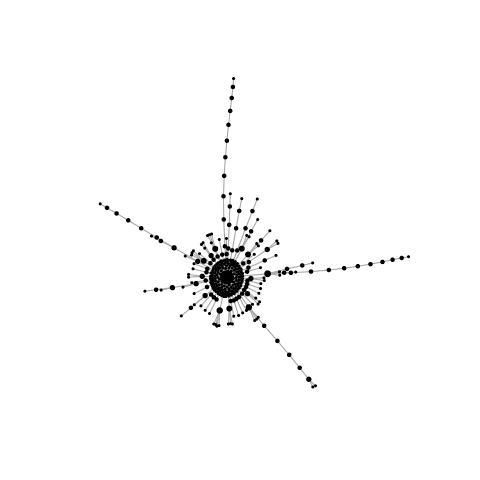
\includegraphics[width=0.32\textwidth]{tree2}
	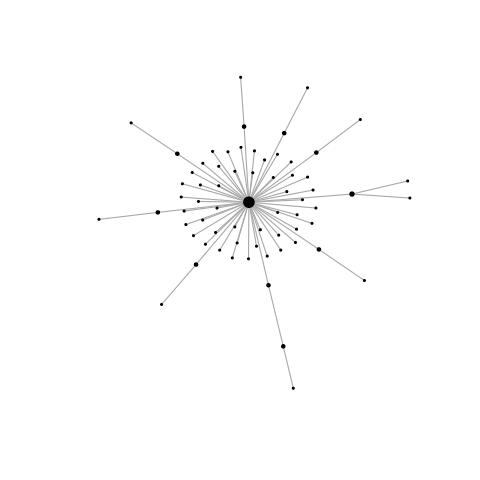
\includegraphics[width=0.32\textwidth]{tree3}
	\caption{Representation of discussion threads with post tree graphs. Vertex represent posts and edges represent replies between posts.}
	\label{fig:trees}
\end{figure}

\section{Neighborhoods in discussion trees}

Our goal is to characterize conversations by their local structure. By local structure we mean the structure of the graph that surrounds a given post, which we call \textit{neighbourhood}. Given a set of posts written by a user, analysing the neighbourhoods where user posts are embedded will give us an insight of what kind of user she is. It is important to note that, if the space of possible neighbourhoods is too small, we might not be able to say anything interesting, while if it is too large we might have neighbourhoods that correspond to the same type of conversation.

In this section, we discuss about the convenience of the classic neighbourhood definition in dynamic graphs such as discussion trees. Then we introduce a new definition to overcome some of the limitations of the classic one when dealing with temporal trees.

\subsection{Structural neighborhoods in discussion trees}

\begin{definition}
Given a tree graph $G$, the \textit{structural neighbourhood} of radius $r$ of post $i$, denoted as $\mathcal{N}_i(r)$, is the induced graph composed of all the vertices that are at distance equal or less than $d$ from post $i$.
\end{definition}
%The above definition is an extension of the classic definition of \textit{neighbourhood} which only considers adjacent vertices.

% pros and cons
The above definition has two drawbacks when used in the context of conversation trees.
%%% not all dynamics are captured
First, the dynamics of the conversation (time or order in which posts are attached to the tree) are not entirely captured in the structure of a tree representation. We know, for instance, that the time in which a node was attached to the tree is always posterior to that of its parent. But it impossible to say, by just looking at the structure of the tree, the order in which a set of sibling posts replied to their common parent post. Since these siblings may get more replies themselves, a single \textit{structural neighbourhood} may sometimes correspond to very different dynamics (see Figure).
%TODO: ejemplo artificial para demostrar que la definicion de vecindario estructural puede corresponder a dinamicas muy diferentes.
%% unbounded size
Second, a structural neighbourhood at a given radius $r$ has an unbounded number of posts, and therefore the space of possible neighbourhoods is infinite. This poses a problem when trying to categorize conversations since many conversations, while structurally different, can be considered semantically equivalent (see Figure)

\begin{figure}
	\centering
	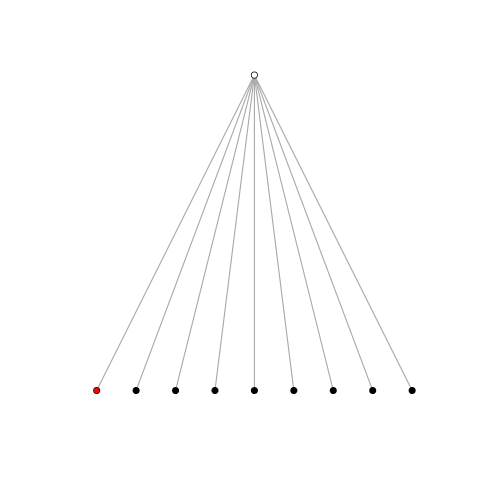
\includegraphics[width=0.4\textwidth]{large_neighborhood}
	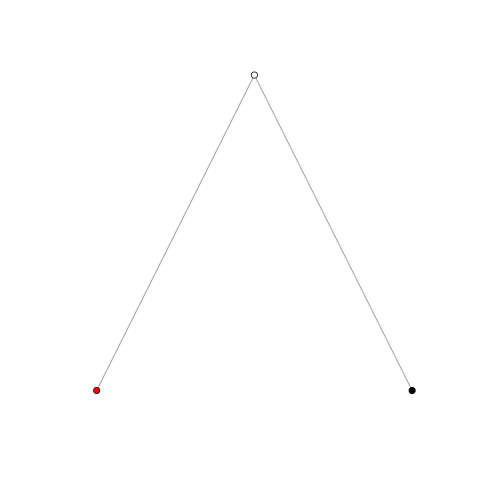
\includegraphics[width=0.4\textwidth]{small_neighborhood}
	\caption{The size of the neighbourhood with radius $r$ is unbounded. These two graph represent frequent neighbourhoods of a post (red) that replied to the root (white). However, the tree in the left corresponds to a very successful root while the three in the right has not brought the attention of too many users.}
	\label{fig:large_neighbourhood}
\end{figure}


\subsection{Structuro-temporal neighborhoods in discussion trees}
\begin{definition}
Given a tree graph $G$, the \textit{structural-temporal neighborhood} of distance $d$ of post $i$, denoted as $\mathcal{N}_{i}^T(r,n)$ is the induced subgraph from its structural neighborhood composed the $n$ vertices that are closer to $i$ in time and for which there exists a path to $i$ in $\mathcal{N}_{i}^T(r,n)$.  
\end{definition}

The above definition has two advantages over the previous one. First, dynamics are better taken into account since the neighbourhood only includes posts that are structurally and temporally close. Second, the size of the neighborhood has an upper bound of $max(\mathcal{N}_i(r)), o)$.

Note that this definition does not consider the timestamp of posts but only the order in which they arrived. An alternative definition of structural-temporal neighborhood might include not the $o$  posts that are closest to the ego post, but every post $j$ at distance $|t_i-t_j|<\tau$ from the ego post $i$. However, both options consider that the local dynamic ends at a fixed horizon ($o$ or $\tau$). This is specially problematic for the case of $\tau$ since different conversation threads may grow at different speeds, as well as different parts of the same thread or even the same part of the thread at different moments (e.g. threads barely grow at night). If we were to use $\tau$ as temporal horizon, we need a mechanism to automatically decide the proper $\tau$ for every post. 

\begin{definition}
Let $s={p^{(1)},...p^{(m)}}$ be the sequence of posts in the structural neighbourhood $\mathcal{N}_i(r)$ ordered by their temporal distance to $i$. Let $\pi=\{\Delta t_1,...,\Delta t_M\}$ be the sequence of time differences between a post in $s$ and its predecessor in $s$. The \textit{temporal radius} $\tau$ of the neighbourhood is the timestamp of the last post $k$ whose $\Delta t_k$ comes from the same distribution than its predecessors $\Delta t_{k-1},..., \Delta t_{1}$ (an intuition for this definition is given in Figure~\ref{fig:cutpoints})
\end{definition}
 
According to the above definition, to find the temporal radius we need to find the first outlier in a sequence of $\Delta t$. Assuming the $\Delta t_i$ comes from an Exponential distribution, and that its $\lambda$ parameter comes itself from a Gamma distribution, we can exploit this conjugacy and obtain the analytical form of the probability of a given $\Delta t_k$ of belonging to the same distribution than its predecessors:
\begin{equation}
p(\Delta t_k | \Delta t_1,...\Delta t_{k-1})
=
\int p(\Delta t_k | \lambda_{k-1})p(\lambda_{k-1} |\Delta t_1,...\Delta t_{k-1})
=\frac{(\beta + n\overline{x})^{\alpha+n}}{(\beta + n\overline{x}+\Delta t_k)^{\alpha+n+1}}(\alpha+n)
\end{equation}
Details of this derivation are given in the Appendix.

\begin{figure}
\centering
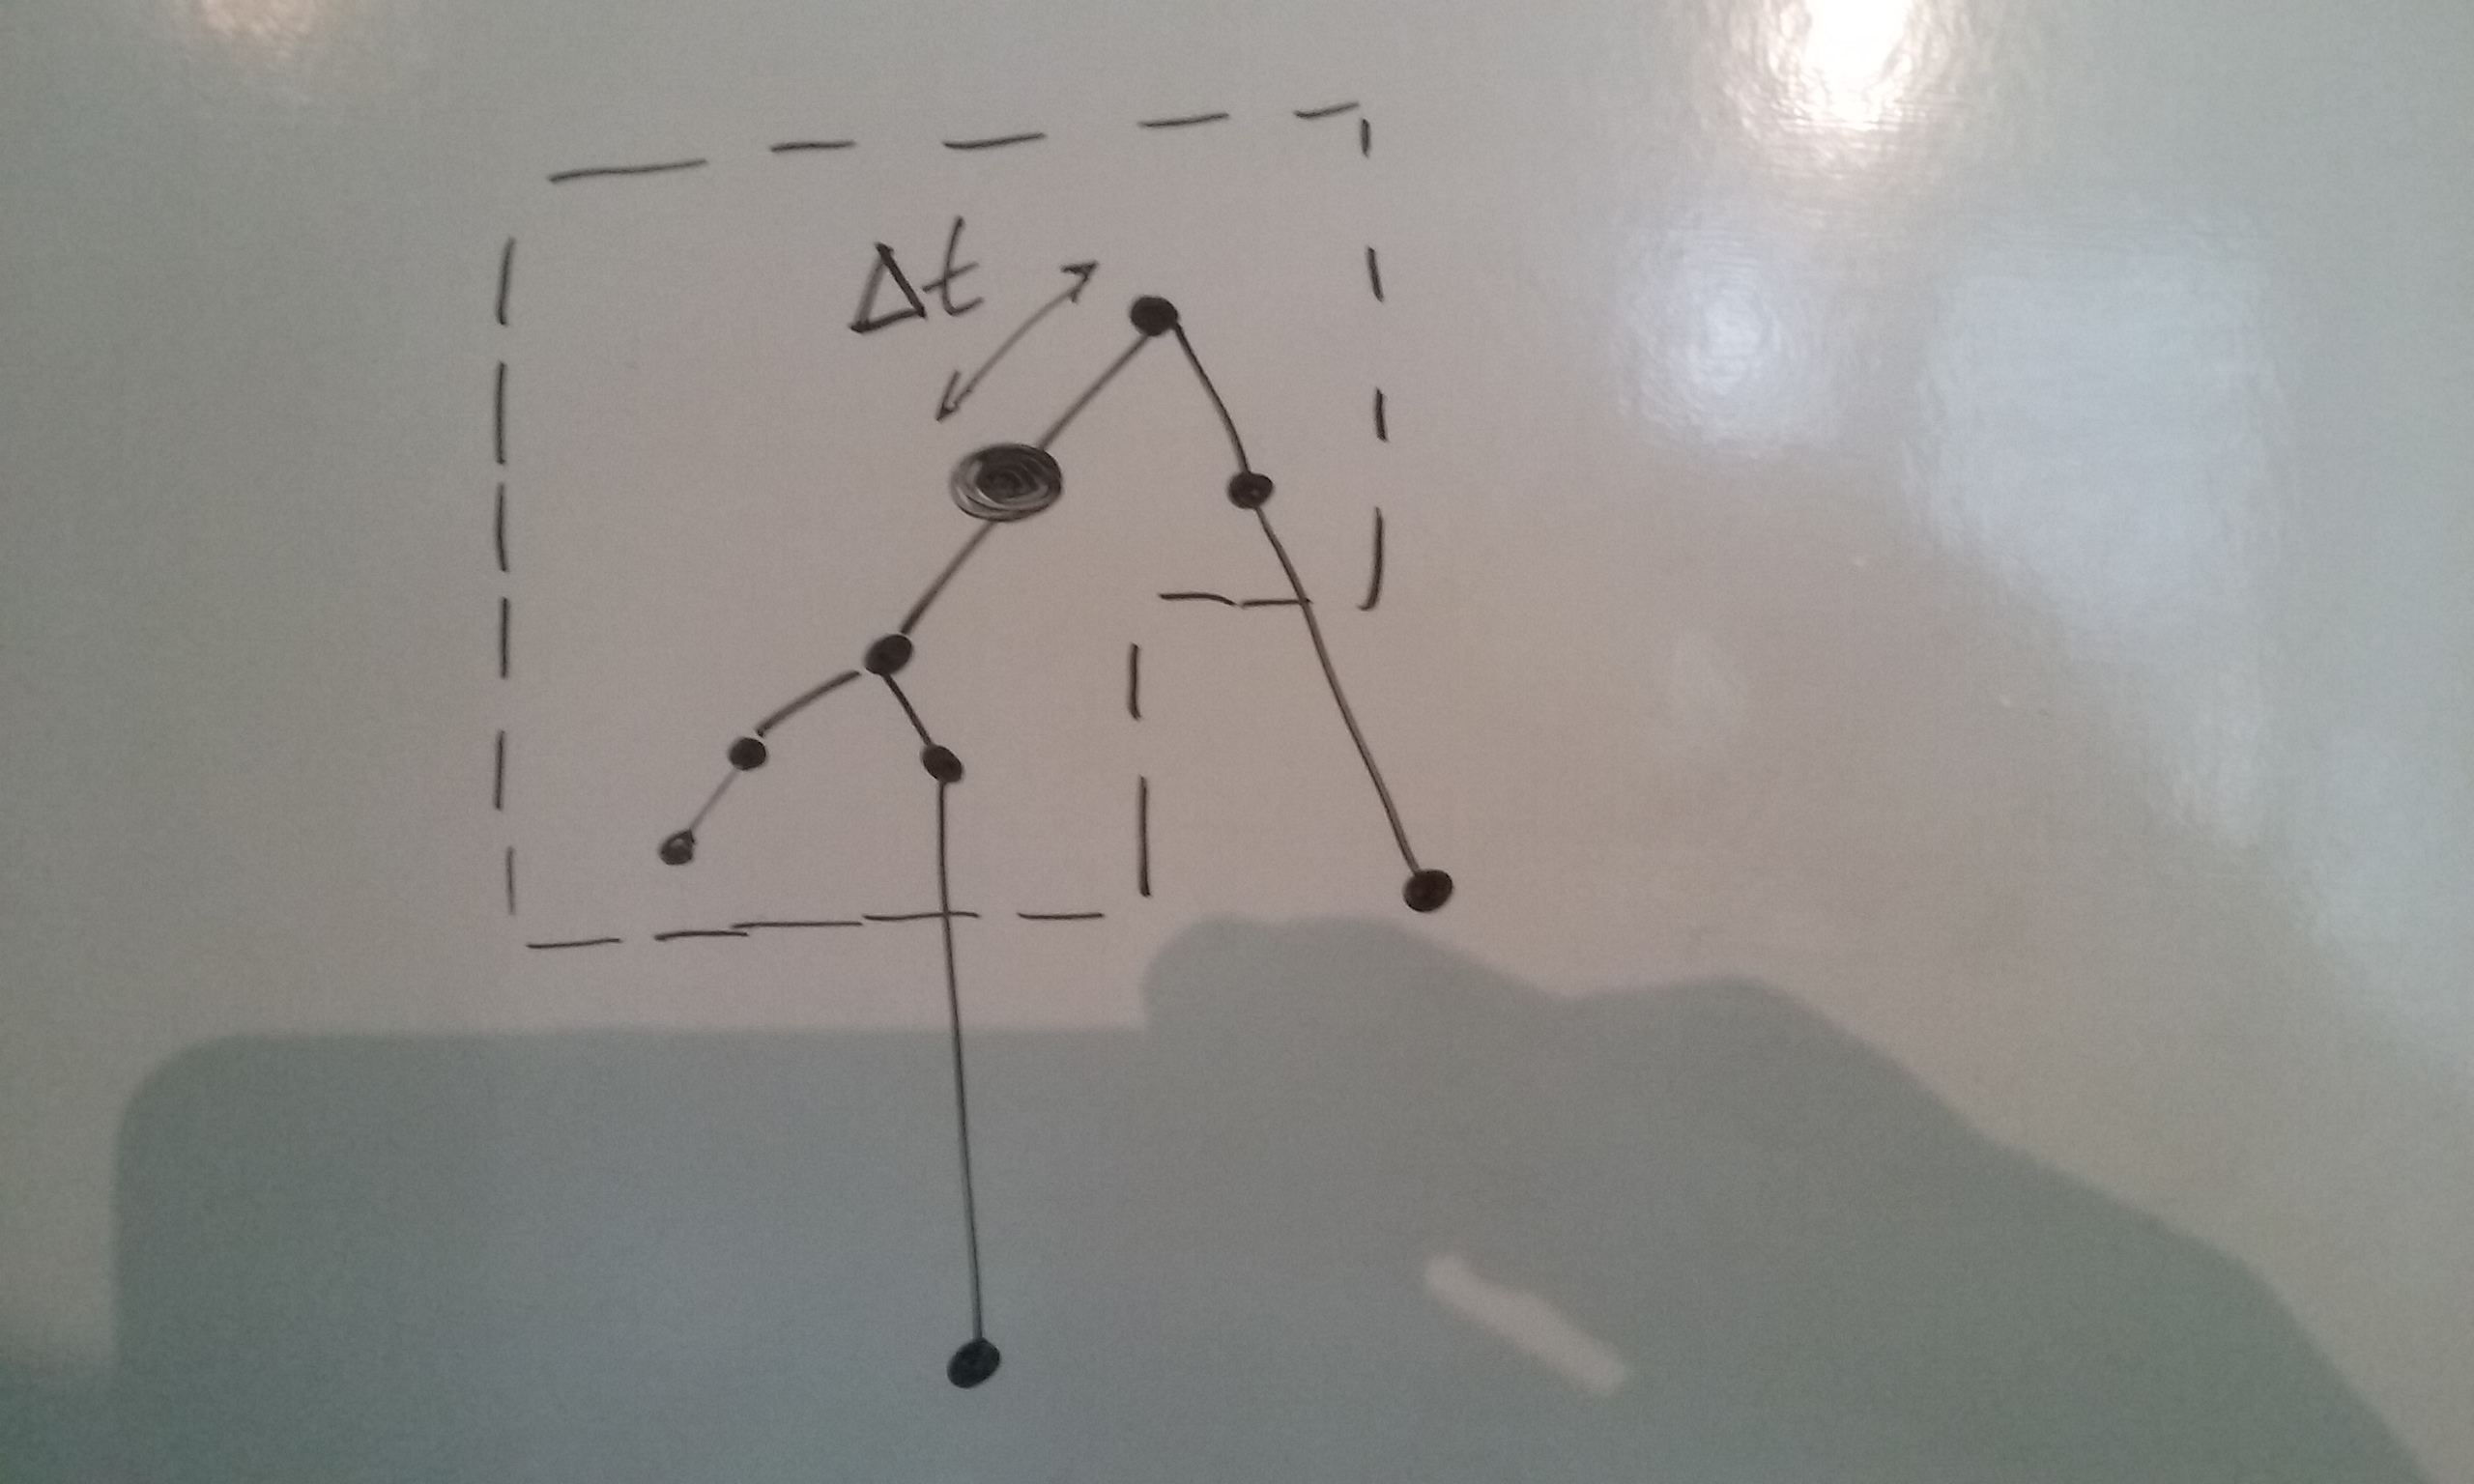
\includegraphics[width=1\textwidth]{temporal_cutpoint}
\caption{Intuition to choice the temporal cutpoint of a neighbourhood. The two posts out of the box have a distance (time) to their parents clearly bigger than the average, so we consider that they are not part of the same local dynamic.}
\label{fig:cutpoints}
\end{figure}

\subsection{Colored neighborhoods}
In conversation trees, the root vertex plays an important role since it represents the post that opened the conversation and thus set the topic of the thread. Therefore, a reply to the root post is clearly different from a reply to any other post in the tree. We distinguish root posts from non-root posts by assigning root posts a unique color (white). We also assign a unique color to the ego post (red). 


\section{Application to Reddit forums}
In this section, we use our definition of structural-temporal neighbourhood to detect different types of users according to the neighbourhoods in which their posts are embedded.

\subsection{Podemos forum}
Our dataset consists of all posts from March 2014 to May 2015 of the Podemos forum in Reddit\footnote{https://www.reddit.com/r/podemos}\footnote{I have also the data for \textit{gameofthrones, france, datascience, machinelearning complexsystems, philosophy, twoxchromosomes, trees, sex}}. The Podemos forum was conceived in March 2014 as a tool for internal democracy, and forum members used it to debate ideological and organizational principles that were later formalized in their first party congress hold in Madrid the October 18th and 19th 2014. Nowadays, its members use it mainly to share and discuss about political news.
The forum contains 83,6119 posts spread over 47,803 threads and written by 26,193 users. (see Figure~\ref{fig:podemos_distributions})

\begin{figure}
\centering
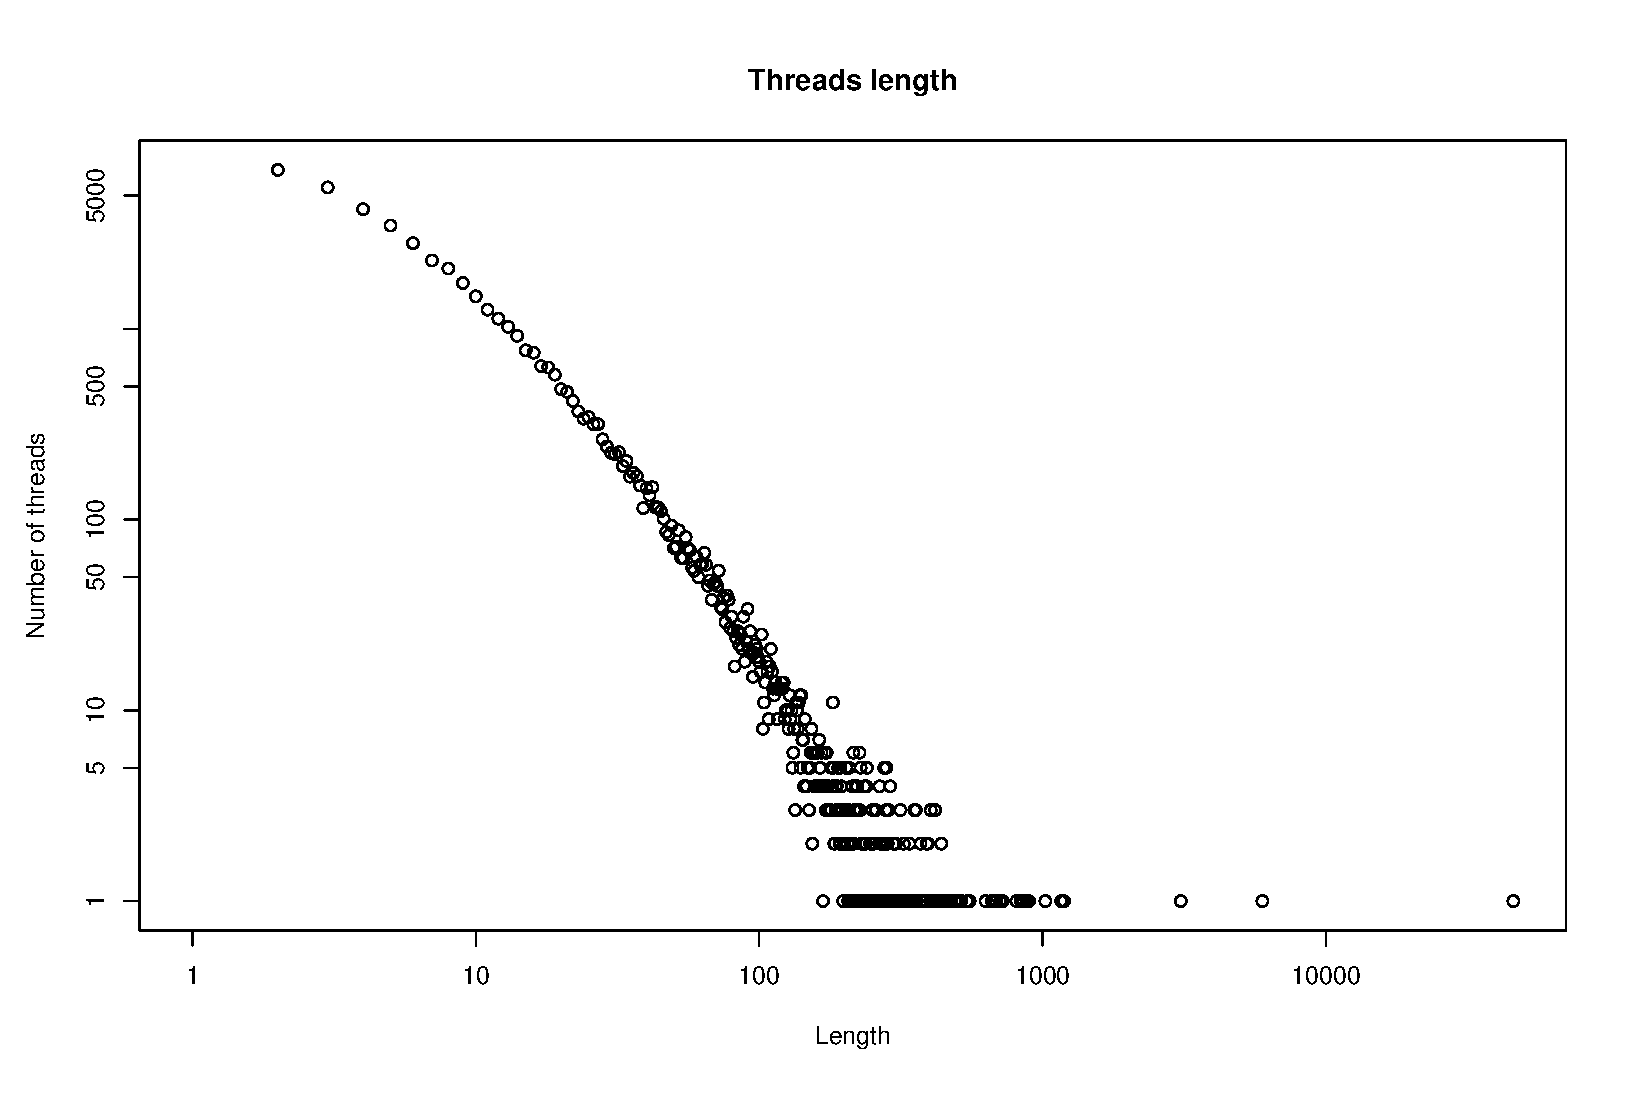
\includegraphics[width=0.5\textwidth]{threads_length}%
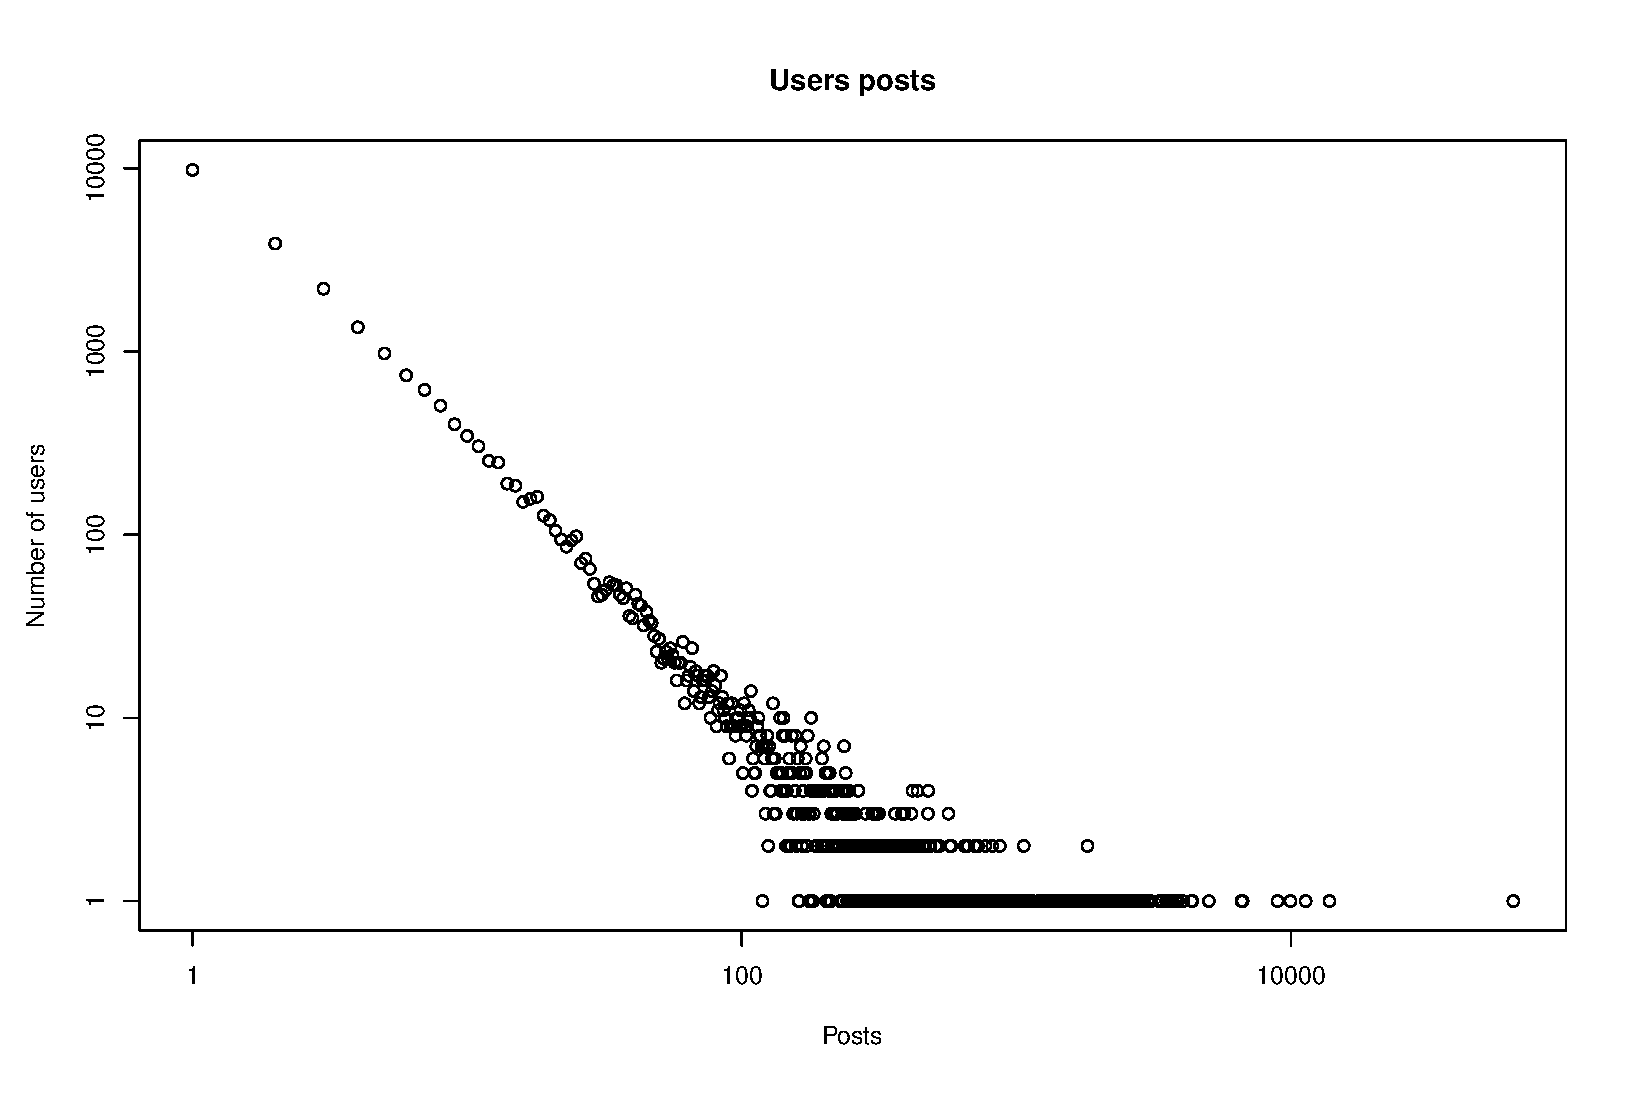
\includegraphics[width=0.5\textwidth]{users_posts}
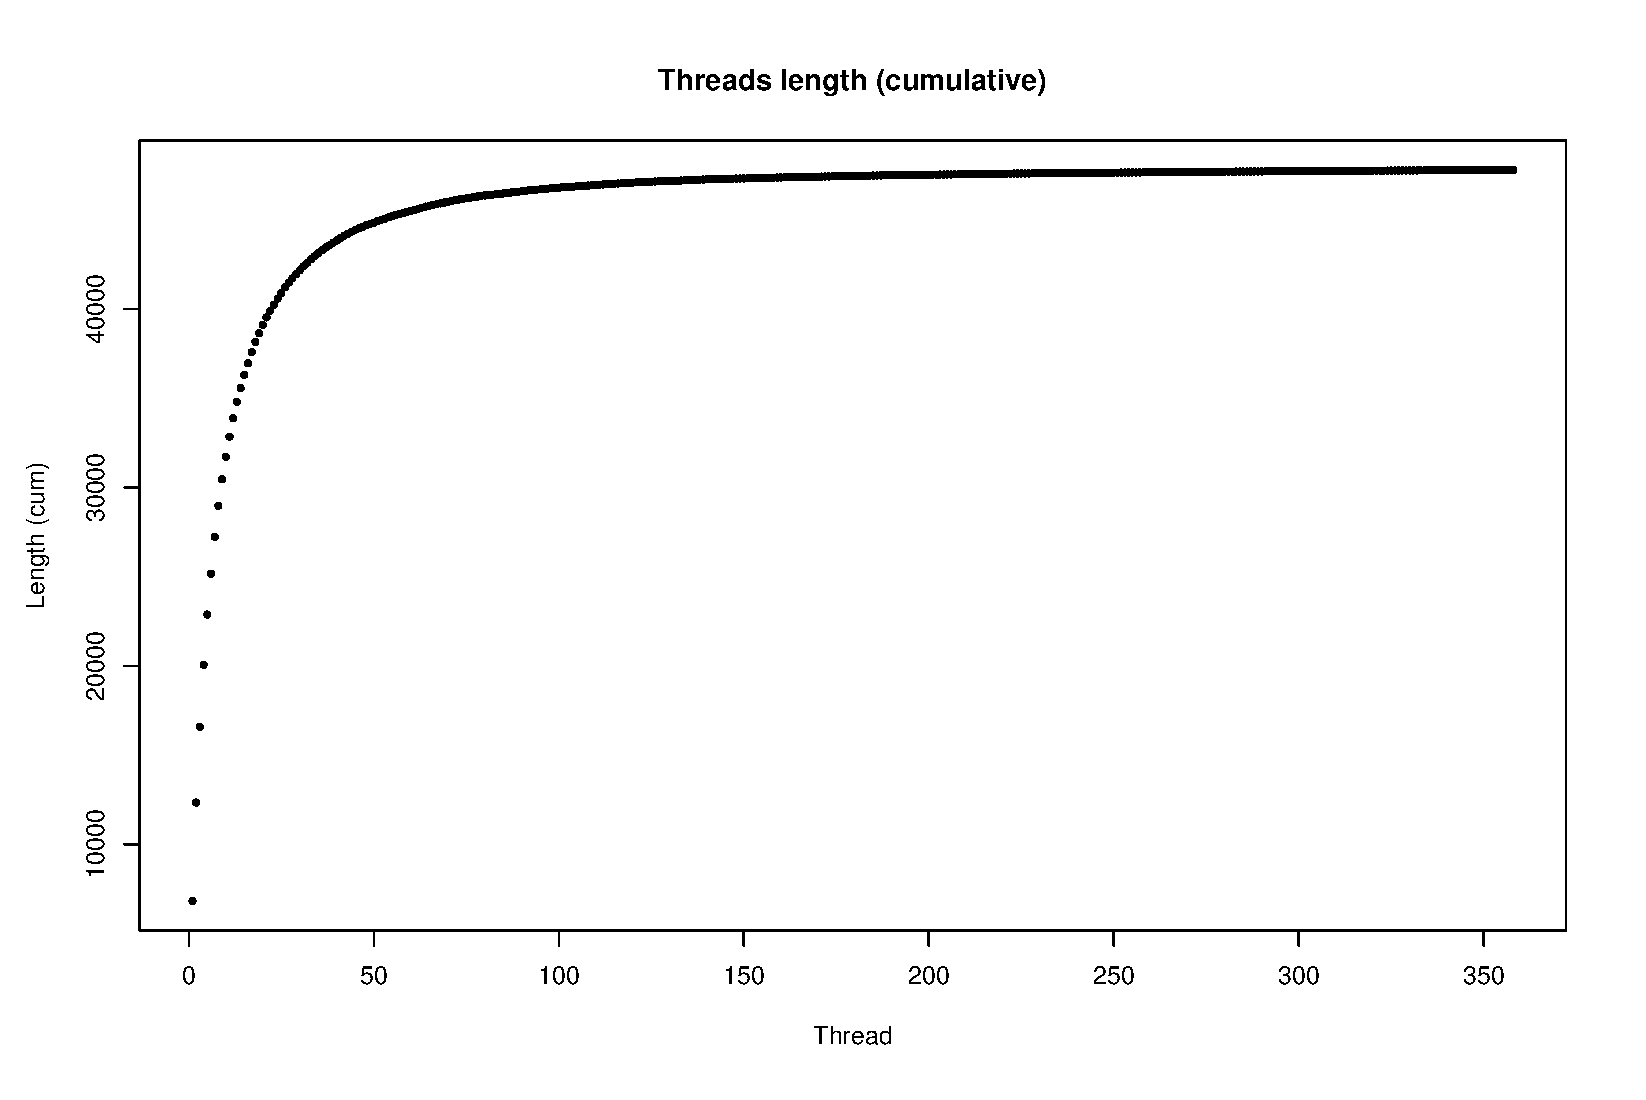
\includegraphics[width=0.5\textwidth]{threads_length_cum}%
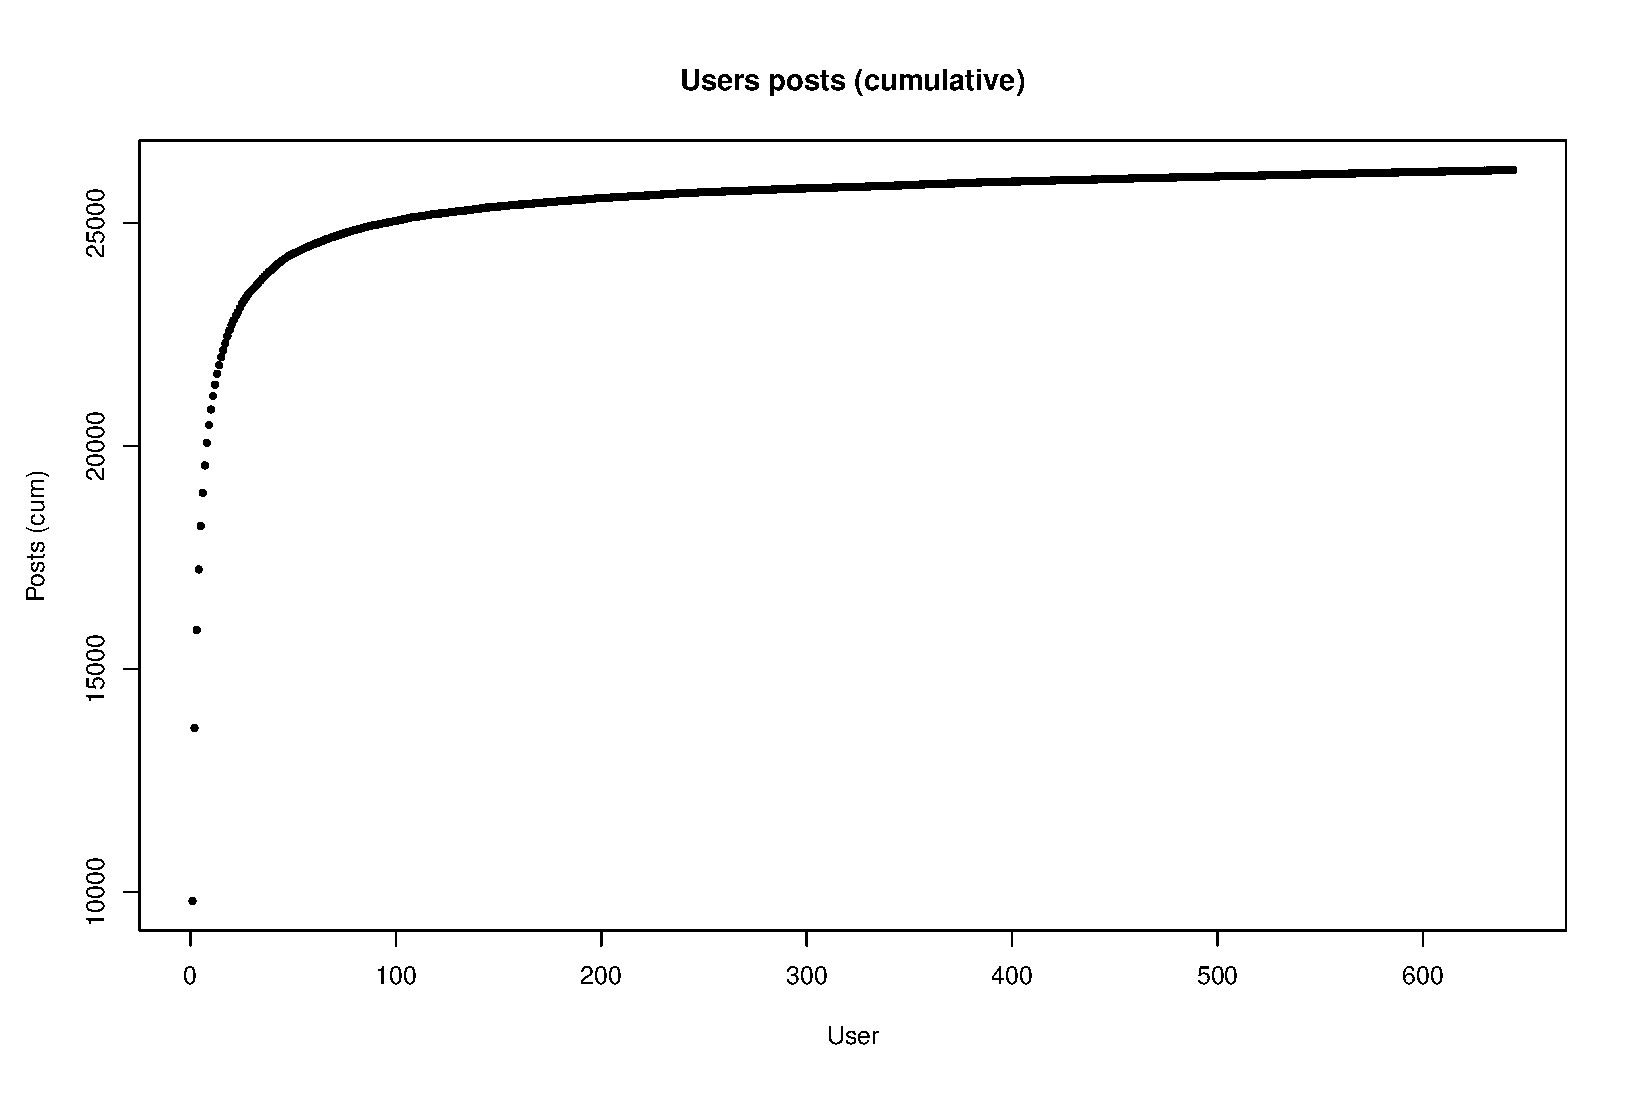
\includegraphics[width=0.5\textwidth]{users_posts_cum}
\caption{Log-log and cumulative distributions and of thread lengths and posts per user.}
\label{fig:podemos_distributions}
\end{figure}

    \noindent\textcolor{red}{\rule{16cm}{1mm}}
(Il fait que j'implemente l'équation 1 pour chercher les neighborhoods. Puis il faut voir si elle sert tout à fait à bien detecter la baisse du rythme)
\subsection{Counting neighorhoods}
In this section we will build a matrix $M$ for one of the forums of Reddit and then we will cluster users to find groups that have similar preferences over the different types of conversations represented by the neighbourhood structures. 

If we set the a spatial radius $r=1$ and an order $n=4$, the temporal neighborhood $N_{G}^{(t)}(i, 1, 4)$ recovers the four adjacent posts that were written temporally closest to a given post. Figure~\ref{fig:neighborhoods_1_4} shows the four detected neighborhoods and their frequency.

In order to detect more complex types of neighborhoods we enlarge the spatial radius to $r=4$. Figure~\ref{fig:neighborhoods_4_4} shows the eight detected neighbors and their frequency. It is interesting to see different structures like chains or stars where the root node migh or might no appear and the ego post is placed at different positions.

\begin{figure}
	\centering
	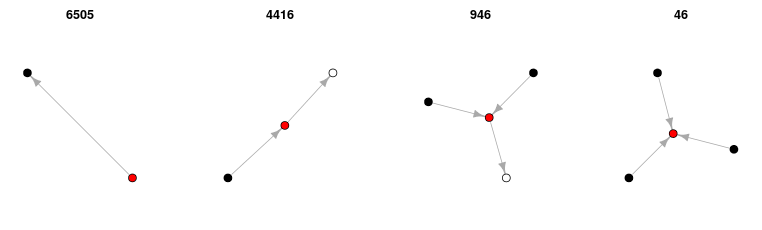
\includegraphics[width=0.8\textwidth]{neighborhoods_1_4}
	\caption{Neighborhood counts with $r=1$ and $n=4$}
	\label{fig:neighborhoods_1_4}
\end{figure}

\begin{figure}
	\centering
	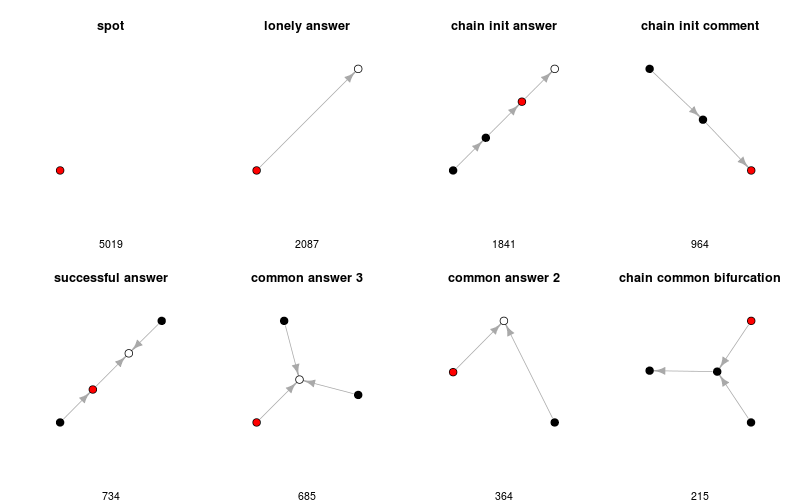
\includegraphics[width=0.8\textwidth]{neighborhoods_4_4}
	\caption{Most frequent neighborhoods with $r=4$ and $n=4$}
	\label{fig:neighborhoods_4_4}
\end{figure}

Note that some neighbors are still very similar. For instance, \textit{common answer 3} is very close to \textit{common answer 2} in the sense that they both represent the ego post replying to a root post that has one and two replies respectively. It seems a good idea to merge them both since they seem to represent the same type of discussion.

\subsection{Clustering}

Given the neighborhoods in which each user participates, we will analyze whether there exists different types of users or all users look similar.

We want to make the analyze independent of the number of posts, and for that we normalize each user feature vector so that features indicate the percentage of posts in this kind of neighborhood. Moreover, some neighborhoods are much more common than others due to the nature of the forums. Thus, we normalize and scale the features so that every feature has a global mean 0 and variance 1. User features now represent z-scores, that is, how many standard deviations is this user feature away from the mean.

We use a simple k-means to find the clusters. To decide the number of clusters, we run k-means for k=2,...,25 clusters and look at the Within-Cluster Sum of Squares (Figure~\ref{fig:elbow}) and we chose $k=5$ so that the results are more interpretable.  Figure~\ref{fig:PCA} shows a PCA projection of the users colored by cluster and the distribution of the clusters in every dimension.
\begin{figure}
	\centering
	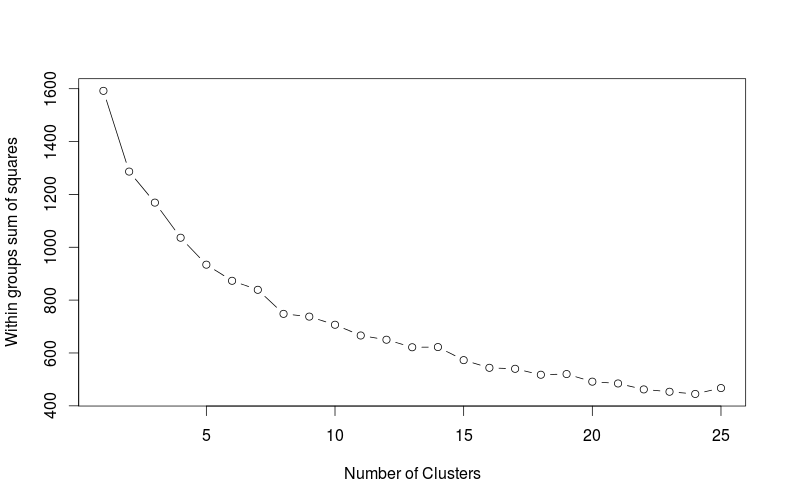
\includegraphics[width=0.5\textwidth]{elbow}
	\caption{Within-Sum of Squares under k-means}
	\label{fig:elbow}
\end{figure}

\begin{figure}
	\centering
	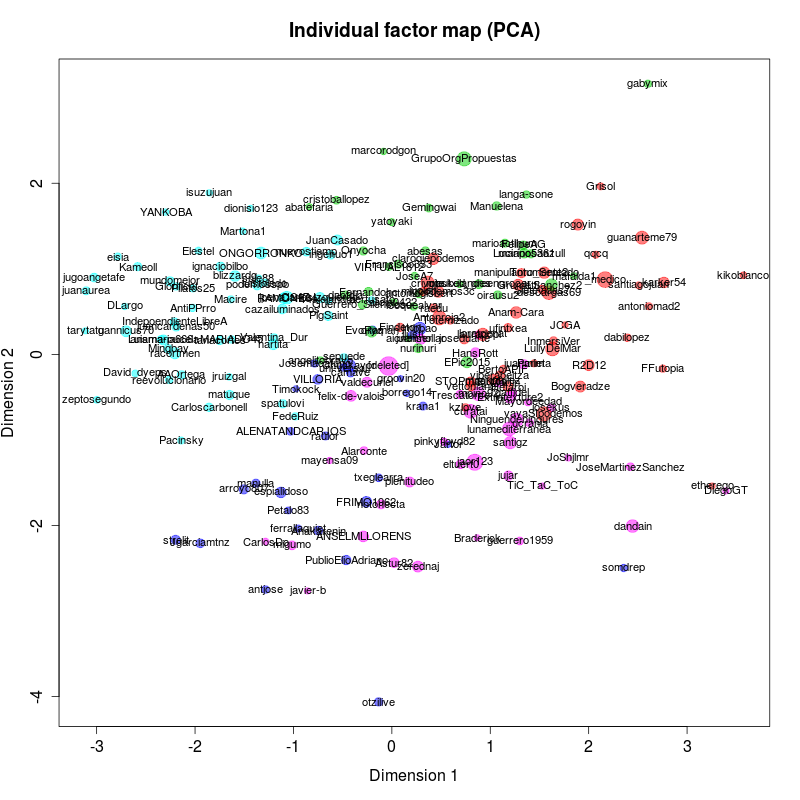
\includegraphics[width=0.5\textwidth]{PCA_nocolor}
	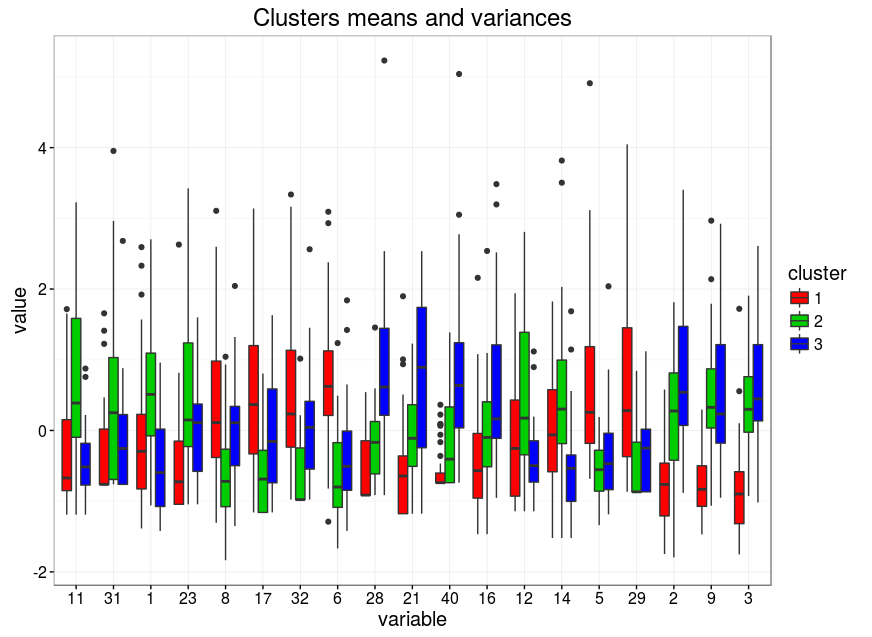
\includegraphics[width=0.5\textwidth]{whiskers}
	\caption{PCA projection of the clusters found and cluster profile in every dimension.}
	\label{fig:PCA}
\end{figure}

\subsection{Predictive roles}
One interesting use of roles is to make predictions on users behaviors. Here, we will analyze whether the initial composition of roles in a thread is a good predictor of the final length of the thread.

\section{Conclusions}
\bibliographystyle{spbasic} 
%\bibliographystyle{chicago} 
%\bibliographystyle{plainnat} 
\bibliography{library}
\end{document}